\chapter{Heat pipe temperature model}

\section{Model derivation}
In greenhouses the effect of a heat pipe ($E$; \si{W/m}) increases with increasing temperature difference between the warmer pipe ($T$; \si{\degreeCelsius}) and the cooler greenhouse air ($T_{air}$; \si{\degreeCelsius}). The effect also increases with pipe diameter (inner diameter: $d$; \si{mm}). The relation can be described empirically by
\begin{equation}
  E=ad\left(T-T_{air}\right)^b
  \label{eq:vg-heat-pipe-E}
\end{equation}
with parameters $a$ and $b$ specific to the pipe material (\iref{fig:vg-heat-pipe-regression}).

\begin{figure} [ht]
\centering
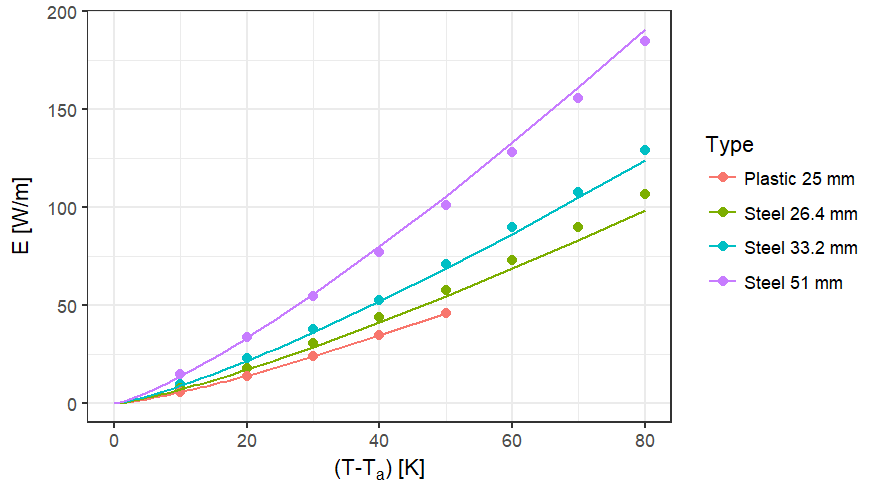
\includegraphics[width=0.67\textwidth]{graphics/vg/heat-pipe-regression.png}
\caption{Regression curves predicting effect ($E$; \si{W} per \si{m} length of pipe) of heat pipes of different materials and diameters \citep[after][Table.~4.3.4]{Braak95}. Curves: $E=ad{\Delta T}^b$. Steel: $a=\SI{0.0154}{\watt\per\milli\meter\per\meter}, b=1.253$. Plastic: $a=\SI{0.0123}{\watt\per\milli\meter\per\meter}, b=1.281$}
\label{fig:vg-heat-pipe-regression}
\end{figure}

The unit of $a$ is \si{W/mm/m} as we ignore the unit of the exponentiated temperature difference. This is a consequence of the equation resulting from empirical data rather than from physical principles.

The energy lost from the pipe at a rate of $E$ \si{\watt\per\meter} (remember that \si{\watt}=\si{\joule\per\second}) results from a cooling of the water it contains. As $T$ drops, in the next instance $E$ will drop as well due to the lessened temperature difference, $T-T_{air}$ (\iref{fig:vg-heat-pipe-regression}). 

Water streams through the pipe; the longer it stays in the pipe, the lower its temperature will drop before it exits. For very long heat pipes or very low flow rates, the temperature of the water, as it exits the greenhouse, will approach that of the greenhouse air ($T_{air}$). Ideally, the temperature of the inflowing water will be regulated to balance the energy lost to the ourdoors environment and to keep $T_{air}$ near the current heating setpoint.

The energy lost from the pipe \eqref{eq:vg-heat-pipe-E} will cause a proportional decrease of the pipe temperature ($T$) determined by the heat capacity (\si{\joule\per\kelvin\per\meter}) of the pipe (water and pipe material). We can then reformulate \cref{eq:vg-heat-pipe-E} as
\begin{equation}
  \frac{dT}{dt} = -kd\left(T-T_{air}\right)^b  
  \label{eq:vg-dT-diff}
\end{equation}
in which $k$ (\si{\kelvin\per\milli\meter\per\minute}) incorporates both $a$ \eqref{eq:vg-heat-pipe-E} and the conversion of the energy loss from \SI{1}{m} of pipe to the corresponding temperature decrease.

If we assume that $T_{air}$ remains constant (\ie\ in a practical setting, it remains close to the setpoint) then we can integrate \cref{eq:vg-dT-diff} over time as 

\begin{equation}
  T(t) = T_{air} + \left[ kd(b-1)t + \left( T(0)-T_{air}\right)^{1-b}  \right]^\frac{1}{1-b} 
  \label{eq:vg-T-integrated}
\end{equation}
where $T(0)$ is the initial pipe temperature at time $t=\SI{0}{s}$, and $T(t)$ is the pipe temperature after the passage of $t$ seconds. 

We now consider the transit time ($\Delta t$) of a small volume of water as it passes through the pipe system. We set the water temperature at the inlet to the initial temperatur $T_{in}=T(0)$ and then compute the temperature of that water volume at the outlet, $T_{out}=T(\Delta T)$. Some typical courses of $T_{out}$ are shown in \cref{fig:vg-heat-pipe-Tout} with $k=\SI{2.5e-6}{\kelvin\per\milli\meter\per\minute}$, $b=1.25$, $d=\SI{37}{\milli\meter}$ and $\Delta t$=\SIrange{0}{30}{\minute}.

\begin{figure} [ht]
\centering
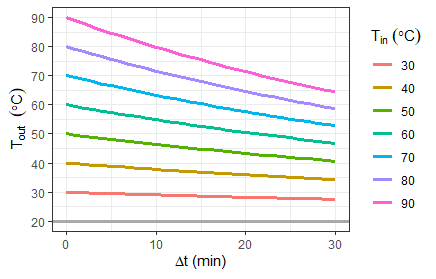
\includegraphics[width=0.67\textwidth]{graphics/vg/heat-pipe-Tout.png}
\caption{Outflow temperature ($T_{out}$) resulting from a range of inflow temperatures ($T_{in}$) and depending on water transit time ($\Delta t$). Air temperature (grey line) fixed at $T_{air}=\SI{20}{\celsius}$. Other parameter values defined in text.}
\label{fig:vg-heat-pipe-Tout}
\end{figure}

\section{Parameter estimation}

Two circuits of heat pipes, top and bottom, were monitored in a greenhouse from 18 April 2018 to 7 August 2019. The pipes were made of carbon steel ($\SI{3}{\milli\meter}$ thickness) with inner diameters $d_{top}=\SI{41.7}{\milli\meter}$ and $d_{bottom}=\SI{43.5}{\milli\meter}$. 

\todo{The equipment} was affixed to the inlet and outlet of both top and bottom pipes. The following variables were logged at a 10-minute interval: water temperature (\si{\celsius}) at inlet ($T_{in}$) and outlet ($T_{out}$), and flow rate ($\dot{V}$; \si{\cubic\meter\per\hour}). A non-linear regression was carried out based on \cref{eq:vg-T-integrated} for each pipe system (top and bottom):
\begin{equation}
  T_{out}(t) = T_{air}(t) + \left[ kd(b-1)\Delta t + \left[ T_{in}(t-\Delta t)-T_{air}(t)\right]^{1-b}  \right]^\frac{1}{1-b} 
  \label{eq:vg-regression}
\end{equation}

The inner diameter ($d$) was fixed at either $d_{top}$ or $t_{bottom}$. The regression analysis was repeated with increasing values of transit time ($\Delta t$) in 1-minute steps, choosing the transit time---for top or bottom pipe---that gave the minimum sum of squared residuals. Since data were available only in \SI{10}{\minute} time steps, intermediate values were derived by linear interpolation. Air temperature would ideally have been constant over the time interval $\Delta t$; it was set to the average during $\Delta t$: 

\begin{equation}
  T_{air}(t)=\left[ T_{air}(t) + T_{air}(t-\Delta t)\right]/2
\end{equation}

Prior to each analysis, data were filtered on four conditions: (i) The pipe water should not have increased in temperature during its transit; (ii) the pipe water should be warmer than the air; (iii) air temperature and (iv) flow rate should be reasonably constant during the period $\Delta t$. Thus only records that lived up to this combined condition were included in any regression:
\begin{align}
\begin{split}
  T_{out}(t) &\leq T_{in}(t-\Delta t)\quad \land \\
  T_{air}(t) &< T_{in}(t-\Delta t)\quad \land \\
  \sigma(T_{air}(t)-T_{air}(t-\Delta t)) &< 3\quad \land \\
  \sigma(\dot{V}(t)) &< 3
  \label{eq:vg-filter}
\end{split}
\end{align}
where $\sigma(x)$ is a function that standardises $x$ to zero mean and unit standard deviation. In effect, all observations outside 3 standard deviations from the average $x$ were discarded.

The delays that yielded the best fit to the regression equation \cref{eq:vg-regression} were $\Delta t_{top}=\SI{15}{\minute}$ and $\Delta t_{bottom}=\SI{23}{\minute}$, respectively (\cref{fig:vg-nordlys-regression}, top row). The best fit was determined by the minimum sum of squared residuals ($SSR$) obtained. This minimum could have arosen due to a smaller sample size (which depended on $\Delta t$ \cf\ \cref{eq:vg-filter}) but there was no trend pointing to particularly low sample sizes around these $\Delta t$ values (\cref{fig:vg-nordlys-regression}, second row). Hence, the estimated $\Delta t_{top}$ and $\Delta t_{bottom}$ were used in the subsequent analysis.

\begin{figure} 
\centering
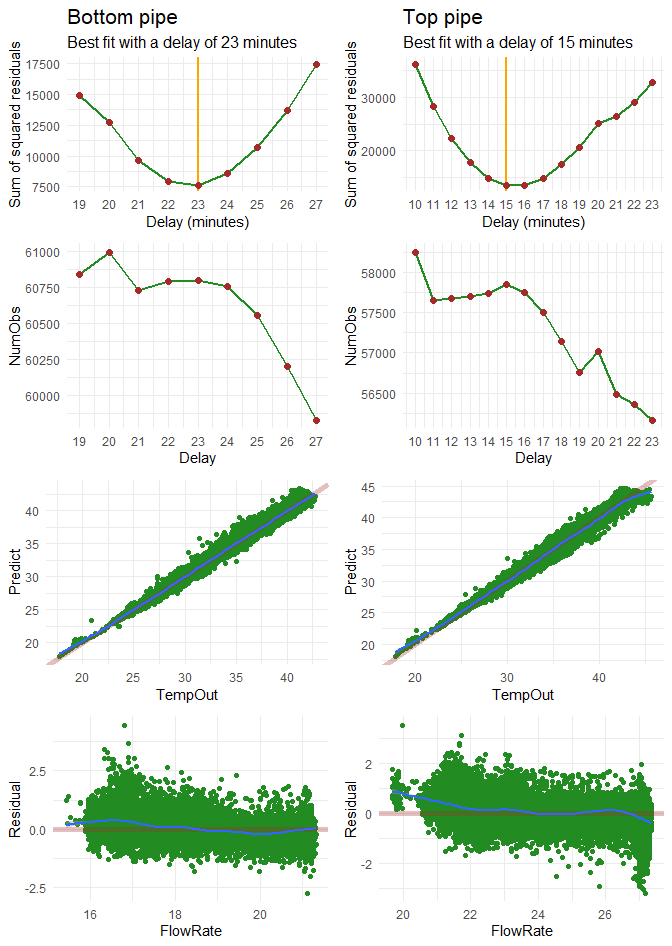
\includegraphics[width=\textwidth]{graphics/vg/vg-nordlys-regression.png}
\caption{Regression analysis of bottom (left) and top (right) heat pipes. First: Sum of residual squares obtained with different delays ($\Delta t$). Second: Number of observations included with different delays. Third: Comparison of observed and predicted outlet temperature ($T_{out}$) overlaid with 1:1 line (brown) and trend curve (blue). Fourth: Regression residual depending on flow rate ($\dot{V}$) overlaid with zero line (brown) and trend curve (blue). Regression in middle and bottom panels carried out with best-fitting delay determined from top panel.}
\label{fig:vg-nordlys-regression}
\end{figure}

\FloatBarrier
Of the original observations (top: \num{68062}, bottom: \num{68672}), many remained after being filter by \cref{eq:vg-filter} (top: \num{57853}, bottom: \num{60801}). The fit was tight and rather unbiased (\cref{fig:vg-nordlys-regression}, third row) with residuals between \SIrange{-2.5}{2.5}{\celsius} (\cref{fig:vg-nordlys-regression}, fourth row).

To check whether the flow rate ($\dot{V}$), which was not included in the regression equation \cref{eq:vg-regression}, could explain the residual variation, scatter plots were inspected and overlaid with trend curves (\cref{fig:vg-nordlys-regression}, fourth row). Visually it was assessed that the variation in $\dot{V}$ was not important for the model. 

The residuals were increasing with the predictor ($T_{out}$) which, together with the temporal autocorrelation of the data and the procedure for choosing $\Delta t$, make the estimated standard errors on the regression parameters ($k$ and $b$) untrustworthy. Hence they are given only as regression point estimates (\cref{tab:vg-regressions}).

\begin{table} [h]
\centering
\caption{Inner pipe diameter ($d$), estimated transit time ($\Delta t$) and coefficients ($k$ and $b$), and sample size ($N$).}
\label{tab:vg-regressions}
\begin{tabular}{lcccc}
Data set & $\Delta t$ (\si{\minute}) & $k$ & $b$ & $N$ \\
\hline
\addlinespace[1.0ex]
Nordlys top    &  \num{15} & \num{2.46e-6} & \num{1.39} & \num{57853} \\
Nordlys bottom &  \num{23} & \num{2.76e-6} & \num{1.23} & \num{60801} \\
\hline
\end{tabular}
\end{table}

The geometry of the pipe system and the measured flow rate provide an alternative calculation of the transit time

\begin{equation}
  \Delta t_{geom} = \frac{V}{\dot{V}}
\end{equation}

The resulting transit times can be seen in \cref{tab:vg-geometry} taking into account the variation in the flow rates ($\dot{V}$).

\begin{table} [h]
\centering
\caption{Pipe inner diameter ($d$), length ($L$) and computed volume ($V$). The \SI{5}{\percent}, \SI{50}{\percent} and \SI{95}{\percent} quantiles of the measured flow rate ($\dot{V}$) and the resulting computed transit time ($\Delta t_{geom}$).}
\label{tab:vg-geometry}
\begin{tabular}{lccccc}
Data set & $d$ (\si{\milli\meter}) & $L$ (\si{\meter}) & $V$ (\si{\cubic\meter}) & $\dot{V}$ (\si{\cubic\meter\per\hour}) & $\Delta t_{geom}$ (\si{\minute})\\
\hline
\addlinespace[1.5ex]

Nordlys top    & \num{36.7} & \num{4394} & \num{4.648} &
  $\begin{pmatrix}  21.48\\ 25.98\\ 27.24 \end{pmatrix}$ &
  $\begin{pmatrix}  12.98\\ 10.73\\ 10.24 \end{pmatrix}$ \\
\addlinespace[2.0ex]

Nordlys bottom & \num{43.5} & \num{5040} & \num{7.490} &
  $\begin{pmatrix}  16.77\\ 20.48\\ 21.14 \end{pmatrix}$ &
  $\begin{pmatrix}  26.80\\ 21.94\\ 21.26 \end{pmatrix}$\\
  
\addlinespace[1.0ex]
\hline
\end{tabular}
\end{table}

\FloatBarrier
\section{Computation of pipe effect}
If we consider a system in steady state with a constant temperature of the water inflow, we can calculate the effect ($P$; \si{watt}) of the pipe. For that we need to know the flow velocity ($v$; \si{\meter\per\second}) and the heat capacity per meter of pipe ($C_{pipe}$; \si{\joule\per\kelvin\per\meter}).

The total length of the heat pipe \cref{tab:vg-geometry} is usually split into $n_{pipe}$ parallel pipes. Thus we get

\begin{equation}
  v = \frac{\dot{V}}{\frac{\pi}{4} d^2 n_{pipe}}
\end{equation}
where $\dot{V}$ (\si{\cubic\meter\per\second}) is flow rate and $d$ (\si{\meter}) is the inner diameter.

We use the heat capacity of water $C_w$=\SI{4181}{\joule\per\kg\per\kelvin} and of steel $C_s$=\SI{502}{\joule\per\kg\per\kelvin} and their densities, $\rho_w$=\SI{1000}{\kg\per\cubic\meter} and $\rho_s$=\SI{7850}{\kg\per\cubic\meter}, to calculate
\begin{equation}
  C_{pipe} = \frac{\pi}{4} \left[ d^2\rho_w C_w + (d_o^2-d^2)\rho_s C_s\right]
\end{equation}
where $d_o$ (\si{\meter}) is the outer pipe diameter
